
%% LyX 2.0.3 created this file.  For more info, see http://www.lyx.org/.
%% Do not edit unless you really know what you are doing.
\documentclass[english, a4paper,11pt]{article}
\usepackage[T1]{fontenc}
\usepackage[latin9]{inputenc}
\usepackage{setspace}
%\usepackage{geometry}
%\geometry{verbose,tmargin=2.5cm,bmargin=2.5cm,lmargin=2.5cm,rmargin=2.5cm}
\setlength{\parskip}{\bigskipamount}
\onehalfspacing
\setlength{\parindent}{0pt}
\usepackage{float}
\usepackage{natbib}
\usepackage{rotating}
\usepackage{graphicx}
\addtolength{\oddsidemargin}{-.875in}
	\addtolength{\evensidemargin}{-.875in}
	\addtolength{\textwidth}{1.75in}

	\addtolength{\topmargin}{-.875in}
	\addtolength{\textheight}{1.75in}
\makeatletter
%%%%%%%%%%%%%%%%%%%%%%%%%%%%%% User specified LaTeX commands.
                           
                                        
\usepackage{array}                                          
\usepackage{longtable}                                       
\usepackage{calc}                                            
\usepackage{multirow}                                         
\usepackage{hhline}                                          
\usepackage{ifthen}                                           
%%  optionally (for landscape tables embedded in another document): 
 \usepackage{lscape} 
\def\inputGnumericTable{}  
\makeatother

\usepackage{babel}
\begin{document}
 
   
\title{Noise Traders or Smart Money? Evidence on Large Participants in the Foreign Exchange Futures Market}
\author{Terry O Malley \\ 12254448}
\maketitle

\section{Introduction}
Best to leave this until the end I reckon. 

\section{Literature Review}

Maybe write this up quickly later in the week.

\section{Data}

The goal of this thesis is to empirically asses a smart money- noise trader model in the foreign exchange market. 

The first piece of data collected is prices of futures contracts. This data is easily attainable from Thomson-Reuters EcoWin Pro, which is open for access to University students. 

In order to test the smart money- noise trader hypothesis, data is also needed  on positions taken by different groups of traders in the asset in question. Unfortunately most foreign exchange trading occurs over-the-counter and is not transacted through a clearing house; the result being that data on traders' positions is either not collected or is proprietary in nature. There are some data available such as that collected by various central banks in major currency trading locations (NYC, London etc) and also the triennial BIS survey of foreign exchange trading activity. This data consists of mostly sparse, short time series and is therefore not suited to a proper econometric analysis. 

Fortunately for this author however, there is a large market in foreign exchange futures contracts, which are traded on the Chicago Mercantile Exchange and therefore are subject to regulation by the Commodity Futures Trading Commission (CFTC). As part of its mandate the CFTC collects confidential daily data on positions taking by large traders in various futures markets, including foreign exchange. The data is released weekly under the `Traders in Financial Futures (TFF)'. In late 2010 the CFTC released four years of historical data reclassified into the TFF format (i.e. positions data disaggregated by large trader types). This data, along with the data collected since then plus futures price data, forms the basis of this thesis. 

The TFF report contains information on open interest of large traders in large futures markets and separates large traders into four categories (one sell-side and three buy-side): dealer/ intermediary (sell-side), asset manager/ institutional, leveraged funds and other reportables (buy-side). It is important to note that the sell- and buy-side distinctions may not necessarily correlate to each group's actual behaviour in financial markets, but rather their general functions across markets. For example, leveraged funds (buy-side) may take short-positions in futures contracts and dealers (sell-side) may be long this same contract. Table 2 describes the classification of each participant. 
\begin{table}[ht]
\begin{tiny}
 \input{tables/participant}  
\addtocounter{table}{-1}
\caption{Futures Market Participant Classification}
\end{tiny}
\end{table}  

The report lists two variables that are of interest to this thesis for each participant. The first is short positions in futures contracts, and the second is long positions. 

\subsection{Dataset Properties}
The dataset that will be studied in this thesis is a combination of the Thomson-Reuters price data and TFF positions data. The TFF data (long and short positions for each participant) is a weekly time series that runs from the 13th June 2006 to the 31st December 2012. Futures market data on six major currencies is chosen for analysis. They are: Australian dollar (AUD), Canadian Dollar (CAD), Swiss France (CHF), Euro (EUR), British Pound (GBP) and Japanese Yen (JPY). 

The price data (expressed as the cost of one unit of currency in US dollars i.e as an exchange rate\footnote{Price for JPY given in cost in USD of one million units of yen.}) for a futures contracts in each currency is downloaded at weekly intervals to match the positions time series and the two datasets are merge. To form the final dataset on which the econometric analysis is carried out, variables for the net positions for each large participant are created by netting long and short positions of each participant type. At this point another variable is created, a net variable that is an aggregate of all large trader positions in each market.  These net variables, along with the price data, for each of the six currencies constitute the final dataset. A description of the dataset is given below. 


\begin{table}[ht]
\begin{tiny}
 \input{tables/descip}  
\addtocounter{table}{-1}
\caption{des}
\end{tiny}
\end{table}

\subsection{Summary Statistics}

Summary statistics for the dataset are presented in table 3. The time series is made up of 343 weekly observations. It is clear from the sample skewness and kurtosis that the data for the various processes are not normally distributed. This will have implications for correlation analysis later on so is noted at this point. The difference between the scales of the price and position data is also noted. 

\begin{table}
\begin{tiny}
 \input{tables/summ}  
\addtocounter{table}{-1}
\caption{Summary Statistics}
\end{tiny}
\end{table}

\subsection{Pairwise Combinations}


In total there are eight variables in the dataset, one of which is the time index and a second which the currency factor. This leaves six variables containing the data of interest: Price and the position variables. The hypotheses of interest in this thesis can be broken into two sets. Firstly what is the relationship between price and the various net positions of large traders. Secondly what is the interrelationship between the net positions of the large traders. Essentially the analysis will deal with taking different pairwise combinations of the data for each currency and assessing correlation between them. In order to do this, a simple combinatorial algorithm can be used to yield the following matrix of unique pairwise combinations\footnote{The R statistical environment \citep{rstats} is used for the analysis in this paper in its entirety.}. 

\begin{table}[H]
\begin{tiny}
 \input{tables/pairs}  
\addtocounter{table}{-1}
\caption{pairs}
\end{tiny}
\end{table}

The actual results from the algorithm produce 15 results. However I am not interested in the combinations of $net$ and its constituent series, so these 4 results are removed. 


\subsection{Visualisation}

As a first step in answering my research question, I visualise different aspects of the dataset to guide analysis. Firstly I plot a multivariate time series graph\footnote{This method of visualising multivariate time series data is provided by \cite{mvtsplot}.} for the currencies to answer a relatively simple question: Are large traders a homogeneous group in their position-taking? This question is motivated by the \cite{wei1997big} paper, in which those authors use data that does not differentiate between large traders but rather treats them as one uniform group. 

\begin{figure}[h]
\begin{center}
\includegraphics[scale=0.8]{heterogeneity}
\end{center}
\caption{Trader Heterogeneity in the Australian Dollar Futures Market. The large centre pane shows the  net positions  time series, each row is one the margins of this series; $other\_net$, $asset\_net$, $lev\_net$, $dealer\_net$. The series is smoothed using a global spline and represented on a colour scale from purple to green, deep purple being the minimum (a large short position) and deep green being the maximum (a large long position). The panel on the right shows the distributions of the margins and the bottom pane shows the entire smoothed series (which corresponds to the $net$ variable in the dataset).}
\end{figure}

The reader can see the limitations of the aforementioned study from this simple graphic. There are clear differences in how each of the large trader types behave in the market. Noticeable is the tendency for leveraged funds and dealers to take the extreme opposite positions as one another. Indeed the relationship seems to be near perfectly negative. Other reportables and asset managers do not take quite as extreme positions (the summary statistics also show large differences in standard deviations between the groups' positions) and do not seem to be as correlated with the other participants. 

The properties of the time series are also of interest, so as an informal first step to explore the possibility that the series are integrated I plot each below\footnote{The lattice graphics package is attributable to \cite{lattice}}.

\begin{figure}[ht] 
\begin{center}
\includegraphics[scale=0.7]{priceviz}
\end{center}
\caption{Time series for price data.}
\end{figure}

As one might expect - and in the spirit of the random-walk hypothesis of asset prices - the price series all seem to feature a stochastic trend. There is evidence that the price series for JPY is trend stationary though. 

\begin{figure}[ht]  
\begin{center}
\includegraphics[scale=0.7]{positionsviz}
\end{center}
\caption{Time series for positions data. Note that all series have been scaled for visualisation.}
\end{figure}

The positions series look more like stationary process on first inspection, though there are noticeable outliers in the $other\_net$ (red) and $asset\_net$ (orange) series. Next I move onto formal tests to assess the stochastic properties of the data. 


\subsection{Unit Root Testing}

I begin by running Dickey-Fuller regressions on every process in the data and calculating the Dickey-Fuller test statistic \citep{dickey1979}. Results from this test and also from the augmented specification are presented in table 4\footnote{D-F test statistics are reported here to save space in the main body of the text. The full regression results are included in the appendix.}.

\begin{table}[H]
\begin{tiny}
 \input{tables/ADF}  
\addtocounter{table}{-1}
\caption{(Augmented) Dickey-Fuller Test Statistics. The first statistic is the standard Dickey-Fuller statistic and the second from a regression augmented with six lags: $k = (n-1)^{1/3}$.}
\end{tiny}
\end{table}

As expected, the null hypothesis cannot be rejected for the price series: the exception being for the yen which appears to be trend stationary\footnote{An auxiliary regression of this series on a time function results in stationary residuals}. There is evidence that the net series are stationary: the null is rejected in most specifications across currencies at the 5\% significance level. At higher lags the null is rejected at the 10\% level except for the Canadian dollar and Euro. The same roughly applies to the dealer series. Most specifications reject at 10\%. Again the augmented statistic is not rejected for CAD and EUR. The asset series is more problematic, the null is not rejected for AUD, GBP and JPY. From figure 3 though, it is noticeable that there is a possible structural break in the AUD asset\_net series in late 2011. There also seem to be large outliers in the GBP series and a possible structural break in late 2011 in the JPY series. These factors may weaken the power of the tests to reject the null. The tests mostly reject for the lev\_net series also. The augmented specifications do not reject for CAD and EUR. The tests reject for the other\_net series at all specifications except for the augmented regression for GBP.  

It is known that the Dickey-Fuller test can suffer from a lack of power to reject the null hypothesis of a unit root \citep{kpss}. As a second test: the \cite {pptest} test\footnote{Available in the R package `tseries' \citep{tseries}}, is performed on the same data for robustness. Again the null hypothesis here is that the series contains a unit root. The tests fail to reject the null for the price series (the exception being the yen again). The tests do reject the null for most of the positions data however. Again the exception is for the asset\_net series, where there was informal evidence of the possibility that large outliers or structural breaks might weaken the power of the unit root tests further. 

\begin{table}[H]
\begin{tiny}
 \input{tables/pptest}  
\addtocounter{table}{-1}
\caption{Phillips-Perron Test Statistics}
\end{tiny}
\end{table}

The conclusion that I take away from this section is that my prior regarding the properties of the time series were by-and-large correct. The price series do seem to follow a random walk and the positions data are likely to be stationary. There are notable exceptions to both, however, and this is kept in mind as a caveat when assessing correlation in the next section. 


\section{Correlation and Dependence Modelling}

\subsection{Scatterplots}

As a first attempt at understanding any relationships between the variables, scatterplots for every pairwise combination are produced, along with a fitted line. Figure 4 shows a visualisation of the relationships between price and the positions data. Figure 5 shows the relationships between the different positions variables. 

For figure 4 it is noticeable that the fitted line is not always an accurate representation of the data. The results are nonetheless striking. A simple linear relationship shows a negative relationship between net positions of all large traders and price. This result is perhaps surprising, though it would be too eager to draw inference from a simple linear representation. The exception is the yen, where a simple linear function seems to fit the data reasonably well and is in fact positive. For dealer positions the picture is a little clearer. Again a linear model does not fit the data too well, but the relationship is consistent across currencies. Dealer positions seem to be negatively correlated to prices: a surprising results perhaps. A reasonable prior might be that dealers, if any party, might be the most likely to represent smart money in the market. The picture for leveraged fund positions is the opposite. A linear model seems to fit reasonably well and shows a positive relationship between leveraged fund positions and price. Maybe leveraged funds are the smart money in the market. 
The results from asset manager and other reportable positions are less consistent than the previous two. For asset managers a linear model shows a negative relationship for the Australian dollar, positive for the yen and none for the rest. For other reportables the estimated relationship is largely negative, except for GBP where the line of best fit does not seem to represent a good fit in the slightest. At this early stage a picture of the data is forming: leveraged funds are smart money, other reportables are noise traders, asset managers are inconclusive and dealers are also noise traders. The picture of dealers as noise traders does not seem to make sense to this author, and remembering the nature of the dealers role it in the market, it may make sense that dealers are on the wrong side of price movements in one market, while hedging in another. 


\begin{figure}[h]  
\begin{center}
\includegraphics[scale=0.8]{scatter1}
\end{center}
\caption{Scatterplots with fitted lines: price and positions}
\end{figure}
%% optional code for 2 col smaller plot
%> pdf('scatter1.pdf', h=5,w=9)
%> grid.arrange(p1, p2, p3, p4, p5, ncol = 2)
%> dev.off()

The scatterplots in figure 5 show the relationships between the various parties in the futures market. The two rows that stick out are rows 2 and 5. The relationship between leveraged funds and dealers is nearly wholly explained by a simple negative linear relationship. This results was hinted at by the multivariate time series plot of the Australian dollar. It seems that dealers and leveraged funds take the extreme opposite positions to each other. Remembering what was seen in the previous plot, it is tempting to conclude that leveraged funds represent smart money and dealers are not noise traders, but merely facilitate leveraged funds positions in the market. There also appears to be a consistent positive relationship between leveraged fund and asset manager positions, though the relationship is a lot nosier than that between funds and dealers. 


\begin{figure}  [h]
\begin{center}
\includegraphics[scale=0.8]{scatter2}
\end{center}
\caption{Scatterplots with fitted lines: positions}
\end{figure}

\subsection{Measures of Correlation}

I now perform relatively simple formal measures of correlations and tests of hypotheses to judge how reliable inference from the simple scatterplot is. I utilise three procedures in this section. The first is the simplest measure of correlation: Pearson's $k$. I then estimate a non-parametric measure: Spearman's $\rho$. Finally I augment the estimates of Pearson's $k$ by running a least squares regression on standardized variables with robust standard errors. 

Firstly the results from the estimates of $k$ are reported in table 7. The results are quite interesting in that the estimates seem to be consistency across currencies and largely statistically significant. Though Pearson's $k$ is a simple way of estimating the relationships between the variables, there are many reasons to doubt the validity of the estimates. Firstly, as was evidenced in the summary statistics, the data is highly non-normal, thus violating the normality of data assumption required by this measure. Secondly, the price series contain a unit root and so any estimate of $k$ from this sample will not converge to the true correlation but diverge as the sample size increases. A third problem is that $k$ only describes linear relationships, yet as seen previously in the scatterplot: the relationships can rarely be defined as linear. For this final reason, Spearman's $\rho$ is also estimated. This non-parametric estimator is not restricted to estimating linear relationships, though it does require any relationship to be monotonic - a much more feasible assumption for this data. Results are presented in table 8. 

Finally an OLS regression is performed. In most specifications, the differing scales of dependant variables and regressors will lead to low estimates of coefficients. To obtain a sensible estimate of the relationship, all variables are scaled by dividing by their standard deviations. In this method the coefficient of the regressor is the same as Pearson's $k$. To correct for autocorrelation in the residuals (Durbin-Watson tests reject the null hypothesis of no autocorrelation of residuals in all specification), robust standard errors are obtained using the method of \cite{vcovHAC} and p-values calculated. Results of specifications where price is the dependent variable are presented in table 9. Results from the positions regressions are reported in table 10. 

\begin{table}[ht]
\begin{tiny}
 \input{tables/pearson}  
\addtocounter{table}{-1}
\caption{pearson}
\end{tiny}
\end{table}

\begin{table}[ht]
\begin{tiny}
 \input{tables/spearman}  
\addtocounter{table}{-1}
\caption{rho}
\end{tiny}
\end{table}

\begin{table}[ht]
\begin{tiny}
 \input{tables/olsprice}  
\addtocounter{table}{-1}
\caption{ols1}
\end{tiny}
\end{table}

\begin{table}[ht]
\begin{tiny}
 \input{tables/olspositions}  
\addtocounter{table}{-1}
\caption{ols2}
\end{tiny}
\end{table}



\subsection{Dependence Modelling Using Vine Copulas}

A better to way to model the dependence within the processes in the data is to use copula methods. As mentioned previous measures of correlation relied on the assumption that the data is normally jointly distributed. This is not the case for most financial data, and summary statistics showed that this dataset is no exception. Copula functions were first described by \cite{Sklar} as a way of measuring dependence between random variables. Sklar's theorem states that a joint distribution function $F(X)$ can be separated into its univariate marginal distribution functions and a copula function that describes the relationship between them. Where a vector of random variables, $x = [x_1, x_2]'$: 

$$F(x) =  C(F(x_1), F(x_2))$$

There is a rich set of Copula functions to choose from to describe the dependence structure between two marginal distributions, and so this method of determining dependence makes more sense for irregular data such as that used in this thesis. 

A recent advance in copula modelling is that of vine copula methods. Vine copulas allow the modeller to specify a `tree'-like structure within the data and estimate a different copula for each pairwise combination in that tree. This method is perfect for the multivariate data in this thesis (i.e. many variables whose interdependence is of interest). For example a Gaussian copula can be specified for the relationship between price and leveraged fund positions, and a completely different copula e.g. Gumbel copula can be used to model the relationship between leveraged fund and dealer positions. Fortunately this method has recently been implemented as the package $CDVine$ in R by \cite{brechmann2012modeling}. In this section I will follow the methodology of those authors, illustrating with the Australian dollar as an example and then providing empirical estimates of a fourth measure of correlation - Kendall's $\tau$ - based on estimated vine copula structures. 

Firstly the dataset must be transformed to `copula data' i.e. the data must lie on the unit interval. This is achieved by non-parametrically transforming the data using each variables' empirical cumulative distribution function (See figure 6).

\begin{figure} [ht] 
\begin{center}
\includegraphics[scale = 0.75]{ecdf}
\end{center}
\caption{Transformation to copula data. The data in the margins of a pair copula must lie on the interval [0,1]. This transformation is achieved by estimating the CDF (middle panel) and applying this function to the data. This transformation is shown in the third panel. After the transformation, values of $1$ are replaced with $1 - 10^{-10}$ to avoid computational issues. }
\end{figure}

\begin{figure} [ht] 
\begin{center}
\includegraphics[scale=0.8]{contour}
\end{center}
\caption{Contour plot. Above the diagonal are scatterplots of the transformed data. Below are the empirical contour plots. Evidence of dependence is evident between price and asset \& lev\_net. Interdependence among participants is also evident.}
\end{figure}

To asses the dependence structure within the data a C-vine Copula is estimated. This is achieved by specifying a tree structure between pairwise combinations of the data and estimating a different copula for the margins of all these pairs. The structure of the tree is reported in table 12. This structure was chosen manually to fit the structure of the research question i.e. what is price's relationship with participants and what is the relationship between the participants. The first tree therefore asses the former relationship and the rest explore the latter. Also note that the $net$ variable is not included in the tree, as it is a composite of the individual positions data and so it would not make sense to include it. 

\begin{table}[ht]
\begin{tiny}
 \input{tables/cvine} 
 \end{tiny}
\addtocounter{table}{-1}
\caption{C-Vine Structure}
\end{table}

Two C-vine models are estimated by maximum likelihood methods using different pairwise copula families and compared via values of the log-likelihood. The first family of copulas is estimated directly using the CDVine package, which chooses each copula family for the first tree and then proceeds to the next trees one-by-one and estimates the copula based on the conditional pairs. The second family of copulas used is just a simple Gaussian copula for every (conditional) pair. 

\begin{table}[ht]
\begin{tiny}
 \input{tables/select}  
\addtocounter{table}{-1}
\end{tiny}
\caption{Copula Selection}
\end{table}

On the basis of the higher log-likelihood, the second model is chosen and is estimated by joint MLE. The empirical values of Kendall's $\tau$ can then be computed based on a transformation of the copula parameters. To apply this methodology across the six currencies I write an algorithm to estimate the c-vine copula structure, compute the parameters by joint ML and then compute $\hat{\tau}$. The results from this procedure are printed in table 15, and a graphic representation of the C-vine tree is presented in figure 8. 

\begin{table}[ht]
\begin{tiny}
 \input{tables/tau}  
\addtocounter{table}{-1}
\caption{Joint ML empirical estimates of Kendall's $\tau$ based on computed c-vine structure. Please refer to table 11 for a description of the structure.}
\end{tiny}
\end{table}
 

\begin{figure}[ht]
\begin{center}
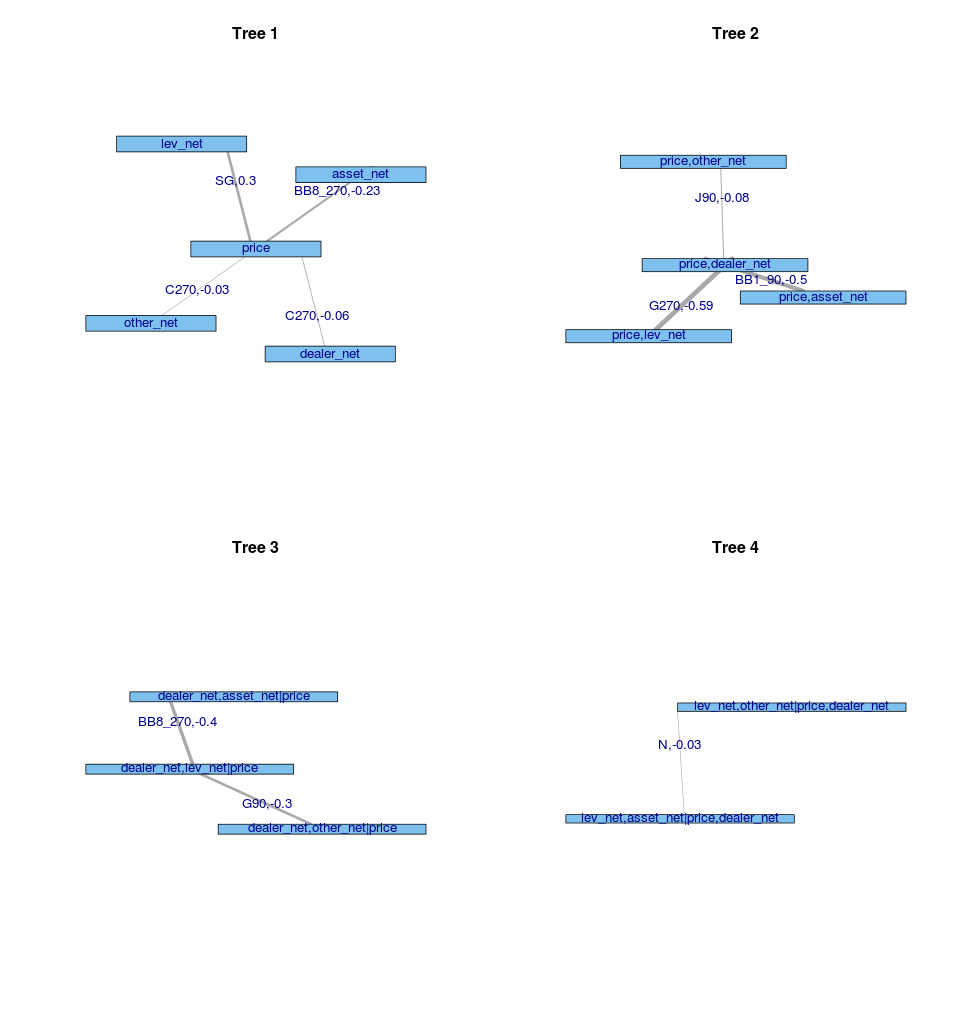
\includegraphics[scale=0.5]{tree.png}
\end{center}
\caption{C-vine tree. Par-copula families and MLE values of Kendall's $\tau$ are reported. The width of each branch is calculated using $\hat{\tau}$. N = Normal (Gaussian) copula, SG = Survival Gumbel copula (Gumbel rotated $180^{\circ}$, F = Frank copula. BB8\_270 = BB8 copula rotated $270^{\circ}$}
\end{figure}

The results confirm what was evidenced by the previous measures of correlation. The relationship between price and dealer positions is negative; between price and leveraged fund positions it is positive and there is weaker evidence for the other two types of large trader. Between participants, there is again a large negative relationship between dealers and leveraged funds, and a slightly less negative relationship between dealers and asset managers. The estimated relationship between asset managers and leveraged funds is negative here interestingly as is the estimated relationship between asset managers and other reportables. 

 
\section{Multivariate Time Series Methods}

The previous section dealt with some topics regarding the dependence structures within the dataset. This section however deals with more specific time series methods. Noticeably lacking from the previous section was any mention of lags. It might be a reasonable position to take that many of the relationships I am interested in exploring in this thesis are dynamic and evolve differently over time, and therefore that the previous section, while helping to illuminate different aspects of the dataset, is not entirely suited to analysis of the dataset. Another issue highlighted in section 3 was that of non-stationarity. The methods used in the previous section cannot be thought of as robust given the non-stationarity of certain processes in the data. Differencing the data would have resolved this problem\footnote{Unit root tests on differenced data confirms.} but information would have been lost in the process.

To demonstrate the above, consider the plot in figure 9 of the empirical cross correlation functions for the Australian dollar. Here price has been first differenced to render it stationary. What is noticeable first is that for the differenced price series, there are no significant cross correlated lags at 0 i.e there is no statistically significant relationship between price and the positions series at lag 0. However lagged correlations between price and positions are significant for net, lev\_net, and dealer\_net. There are none for asset\_net, and significant lags for other\_net for the opposite effect. Already this simple plot gives an idea as to the dynamic properties of the dataset; net, dealer and leveraged fund positions are correlated with prices at negative lags, asset managers price are not correlated and other reportable positions are negatively correlated at positive lags. Already a simple story of the differences in the dynamic behavoiour of each group is revealed. Dealers and leveraged fund positions seem to come before price changes and other reportable position come after. 


To give a better answer to the research question I now turn my interest to how prices and positions behave over time. To test the hypothesis that there is a dynamic relationship between some pairwise combinations of the variables I wish to test for Granger-causality. I adopt the standard vector autoregression (VAR) framework to do so. 
\begin{figure}  [H]
\begin{center}
\includegraphics[scale=0.5]{ccf}
\end{center}
\caption{Cross-Correlation Function. On the x-scale is the time lag between the two series}
\end{figure}


\subsection{Vector Autoregression}

To explore the idea that there may be some dynamic relationship between different pairwise combinations in the data, a reduced-form vector autoregression (VAR) is estimated for each of them. As a result there $6 X 11$ VAR($k$)s to be estimated. Choosing the number of lags, $k$, for each of these VARs is a non-trivial task. The approach I have opted to use involves writing an algorithm sequentially combining functions from the `vars' package in R {\citep{vars}}. The algorithm chooses the 11 relationships of interest for each currency, performs two selection criteria: Akaike information criteria (AIC) and Schwarz- Bayesian information criteria (BIC), and then estimates a VAR($k$) where $k$ is pre-decided by the user as either $$k\,=\,max\{k(AIC), k(BIC)\}$$ or $$k\,=\,min\{k(AIC), k(BIC)\}$$ The reason for this two-step approach (meaning $66 X 2$ VARs) is to eliminate any possibility that a misspecified VAR is giving spurious results. For example AIC and BIC can often determine wholly different estimates of $k$, a large $k$ may result in spurious statistical significance (type I error) and a low $k$ may result in a type II error. 

\subsection{Granger-Causality Tests}

Following this model selection, the algorithm then proceeds to test the hypothesis that one of the variables in the system does not help in explaining the other (standard Granger-causality test). The null hypothesis for this test is of no Granger-causality, which we might expect as a reasonable position consistent with an efficient market hypothesis view of futures contracts prices. 

Results from these tests are presented in tables 14 and 15. Table 14 shows results from VARs estimated on the relationships between prices and participant positions. Table 15 shows results from estimates of relationships between market participants' positions. 

\subsubsection*{Price and Large Trader Positions}
The results from table 14 are indeed noteworthy. They do reveal a pattern of predictability from price to movements in large traders positions. They go a long way in backing up what was demonstrated by the analysis in the preceding section. There is strong evidence across both specifications of the VAR systems that $net$ positions of large traders has power to predict the movement of futures prices. There is strong evidence also that the positions of dealers and leveraged funds both, as individual groups, also have power to predict movements in prices. There is also evidence that, at large lags, asset manager positions help to predict price movements. This result is seen especially in the yen where the previous section showed strong positive dependence between the two series, and also in the Euro. For other reportables the evidence is less strong. There is an indication that other reportables' positions help predict price movements in the British pound, and also for the Canadian dollar. 
\begin{table}[ht]
\begin{tiny}
 \input{tables/granger_price}  
\addtocounter{table}{-1}
\caption{granger}
\end{tiny}
\end{table}

In the direction Granger-causality from price to positions, there is little evidence to suggest net positions Granger-cause prices. At longer lags there null is rejected for EUR and GBP at 10\% but this results is not robust to a short lag specification. The JPY does shows some significance also. There is stronger evidence that prices Granger-cause dealer positions except for the AUD and EUR. Perhaps this is not surprising given the nature of the dealer's role as an intermediary in the market. The evidence is weak to reject the null hypothesis that price Granger-causes asset manager positions. Again there is some evidence that prices Granger-cause leveraged fund positions for CHF, GBP and JPY. For other reportables, again there is some inconsistent evidence across currenices; AUD, CAD and EUR show evidence to reject the null (though there is no evidence for AUD at one lag, this is perhaps a strong restriction to impose). 

\subsubsection*{Among Large Trader Positions}




Unsurprisingly, given what was seen in section 3, there is strong evidence in table 15 to reject the null hypothesis that dealers and leveraged funds positions are not robustly related. There is also evidence that asset manager position cause dealer positions. Neither results may be considered surprising, again given the nature of a dealer's role in the market. There are some rejections of the null for the rest of the specifications but nothing consistent across a number of currencies. 

\begin{table}[ht]
\begin{tiny}
 \input{tables/granger_positions}  
\addtocounter{table}{-1}
\caption{granger}
\end{tiny}
\end{table}

\subsection{Toda-Yamamoto/ Dolado-L\"{u}tkepohl Modified-Causality Tests}

An issue that must be addressed in the preceding section regards the non-stationarity of the price data. The VARs are all estimated in levels to prevent loss of information from first differencing \cite[p. 244]{lutkepohl2005new}. Unfortunately in this case, the asymptotic properties of the test statistic may not be valid under the null \citep{lutkepohl2005new, varsvignette}. Fortunately both \cite{toda1995statistical} and \cite{lutkepohl1996} provide the methodology to test restrictions on a VAR estimated in levels, where some or all of the processes are integrated or cointegrated\footnote{See \cite{lutkepohl2005new} for a textbook treatment.}. To do so the optimal lags $k$ are determined as usual and a VAR with lags $m = k + d_{max}$ is estimated, where $d_{max}$ is the maximum order of integration of the processes in the system. To test restrictions such as the joint restrictions in a Granger-causality test, the usual restrictions can be applied to the first $k$ lagged coefficients and covariance matrices using a Wald test with $k$ degrees of freedom. The $\chi^{2}$ test statistic is then asymptotically distributed under the null.

I carry out this analysis for the price and position VAR systems and present the results in table 16\footnote{R package `dynlm' \citep{dynlm} is used to estimate the linear relationships and `aod' \citep{aod} is used to test the appropriate linear restrictions.}. The conclusions from the non-corrected tests largely remain. $Net$, $lev\_net$ and $dealer\_net$ all show strong evidence that they have the power to predict prices. There are also many rejections of the null for $asset\_net$ and only 1 for $other\_net$ at the 5\% significance level. 

There is little evidence of Granger-causality in the opposing direction in these tests. Though there are some strong rejections of the null, only is robust across both specifications (dealer\_net | AUD) 


\begin{table}[ht]
\begin{tiny}
 \input{tables/ty_price}  
\addtocounter{table}{-1}
\caption{typrice}
\end{tiny}
\end{table}

\subsection{Sub-sample Robustness}

As a test for robustness, the preceding VAR analysis is carried out again. This time the models are estimated on three sub-samples of the data with $k$ chosen only according to BIC for brevity. The first runs from 02-11-2010 to 31-12-2012. The second from 19-08-2008 to 26-10-2010 and the third from 13-06-2006 to 12-08-2006. The results from these specifications are reported in tables 17 and 18. The results show a more robust conclusion that $dealer\_net$, $lev\_net$ and $net$ are all helpful in predicting price, and that $dealer\_net$ is helpful in predicting $lev\_net$. 

\begin{table}[ht]
\begin{tiny}
 \input{tables/sub_price}  
\addtocounter{table}{-1}
\caption{sub}
\end{tiny}
\end{table}

\begin{table}[ht]
\begin{tiny}
 \input{tables/sub_positions}  
\addtocounter{table}{-1}
\caption{sub}
\end{tiny}
\end{table}

\subsection{Impulse Response Functions}

Now that Granger-causality relationships have been established, it would be useful to determine how exactly the processes react to a shock in another. Impulse response functions are calculated based on a VAR(3) and are plotted below. 


%%%%%%%%%%%%%%%%%%%%%%%%%%%%%%%%%%%
%%% Impulse Response Functions %%%%
%%%%%%%%%%%%%%%%%%%%%%%%%%%%%%%%%%%

\begin{figure}  [ht]
\begin{center}
\includegraphics[scale=0.25, page=1]{irf}
\includegraphics[scale=0.25, page=2]{irf}

\includegraphics[scale=0.25, page=3]{irf}
\includegraphics[scale=0.25, page=4]{irf}

\includegraphics[scale=0.25, page=5]{irf}
\includegraphics[scale=0.25, page=6]{irf}

\includegraphics[scale=0.25, page=7]{irf}
\includegraphics[scale=0.25, page=8]{irf}

\includegraphics[scale=0.25, page=9]{irf}
\includegraphics[scale=0.25, page=10]{irf}
\end{center}
\caption{sample IRF, price net}
\end{figure}

\begin{figure}  [ht]
\begin{center}

\includegraphics[scale=0.25, page=11]{irf}
\includegraphics[scale=0.25, page=12]{irf}

\includegraphics[scale=0.25, page=13]{irf}
\includegraphics[scale=0.25, page=14]{irf}

\includegraphics[scale=0.25, page=15]{irf}
\includegraphics[scale=0.25, page=16]{irf}

\includegraphics[scale=0.25, page=17]{irf}
\includegraphics[scale=0.25, page=18]{irf}


\includegraphics[scale=0.25, page=19]{irf}
\includegraphics[scale=0.25, page=20]{irf}


\includegraphics[scale=0.25, page=21]{irf}
\includegraphics[scale=0.25, page=22]{irf}
\end{center}
\caption{sample IRF, price net}
\end{figure}


\section{Conclusion}

\bibliographystyle{apalike}
\bibliography{mybib}

\end{document}
